\documentclass[12pt]{article}
\usepackage[portuguese]{babel}
\usepackage[utf8]{inputenc}
\usepackage[usenames,dvipsnames]{color}
\usepackage{setspace}
\usepackage{amsmath}
\usepackage{amsfonts}
\usepackage{amssymb}
\usepackage{mathtools}
\usepackage[top=3cm, bottom=2cm, left=3cm, right=2cm]{geometry}
\usepackage{tikz}
\usepackage{indentfirst}
\usepackage{textcomp}
\usepackage{float}
\usepackage[font={small,it}]{caption}
\usepackage{mhchem}
\usepackage{algpseudocode}
\usepackage[plain]{algorithm}

\title{Relatorio Final Mestrado}

% packages added by Marcelo
%
\usepackage{lscape}    % for landscape pages
\usepackage{hyperref}  % to allow hyperlinks
\usepackage{booktabs}  % nicer table borders
\usepackage{subfigure} % add subfigures

% My default commands
\newcommand{\foreignword}[1]{\textit{#1}}
\newcommand{\toolname}[1]{\textit{#1}}
%\newcommand{\fieldR}{\mathbb{R}}
\newcommand{\powerset}{\mathcal{P}}
%\newcommand{\probability}{\mathbb{P}}
\newcommand{\expectation}{\mathbb{E}}
\newcommand{\algname}[1]{\texttt{#1}}
\newcommand{\langname}[1]{\texttt{#1}}
%\newcommand{\varname}[1]{\texttt{#1}}
%\newcommand{\floor}[1]{\lfloor #1 \rfloor}
%\newcommand{\ceil}[1]{\lceil #1 \rceil}
%\newcommand{\mathsc}[1]{{\normalfont\textsc{#1}}}
\newcommand{\forest}{\mathcal{F}}
\newcommand{\pfsnode}[1]{\mathbf #1}
\newcommand{\species}[1]{\textit{#1}}
\newcommand{\gender}[1]{\textit{#1}}

\graphicspath{{./img/}} 

\setstretch{1.5}

\begin{document}

% FAPESP demands the usage of double spacing
%
\doublespacing

\begin{titlepage}
    \vfill 
    \begin{center}
        {\Large Relatório Científico Final -- Mestrado\\
         \bigskip
         Processo FAPESP 17/20575-9
        }
        
        \bigskip
        \bigskip
    
        {\LARGE Identificação de vias de sinalização celular baseada em
        repositórios de cinética de reações bioquímicas}

        \bigskip
        \bigskip
        {\Large {\bf Beneficiário:}
        \href{mailto:gustavo.estrela.matos@usp.br}{Gustavo Estrela de
        Matos}\\ 
        
        {\bf Responsável:}
        \href{mailto:marcelo.reis@butantan.gov.br}{Marcelo da Silva
        Reis}\\

        \bigskip
        \bigskip
        \bigskip
        \bigskip
        \bigskip
        \bigskip
        \bigskip
        Relatório referente aos trabalhos desenvolvidos entre 10 de
        dezembro de 2018 e 31 de dezembro de 2019

        \bigskip
        \bigskip
        \bigskip
        \bigskip
        \bigskip
        \bigskip
        \bigskip

        Laboratório Especial de Toxinologia Aplicada, Instituto
        Butantan\\
        \bigskip
        São Paulo, \today\\
        }

        \bigskip
        \bigskip

       

\end{center}
\end{titlepage}


\tableofcontents

\pagebreak



\section{Resumo do Projeto Proposto} \label{sec:resumo} % até 2 páginas
A construção de modelos funcionais é uma técnica comum para se 
estudar vias de sinalização celular e, quando a via estudada é pouco
conhecida, é possível que os modelos já propostos sejam incompletos, 
tornando necessário a sua modificação.
Lulu Wu apresentou em 2015, em sua dissertação de mestrado, um método 
para  modificar sistematicamente modelos funcionais, adicionando a estes
interações extraídas de repositórios como KEGG. Entretanto, esta 
metodologia apresentou limitações: a primeira é a incompletude do banco 
de dados de interações criado, que extraia informações apenas do 
repositório KEGG; a segunda, a falta de informações sobre constantes 
de velocidade de interações, que podem ser extraídas de repositórios 
como BioNumbers; a terceira, a dinâmica do algoritmo de busca, 
incremental, que pode não achar o mínimo global; e a última, a 
penalização na complexidade dos modelos, que era feita de maneira 
aleatória. Propomos neste trabalho enfrentar as limitações encontradas
pela metodologia de Lulu, criando um banco de dados de interações mais
completo e também novas funções de custo que sejam capazes de 
penalizar modelos mais complexos (como critério de informação Akaike e 
{\em Bayesian inference-based modeling}); esta penalização deve induzir,
em cadeias do  espaço de busca, curvas em u no custo dos modelos, 
portanto também propomos a criação de novos algoritmos de busca que 
explorem essa característica da função de custo. Por fim, esperamos 
testar nossa metodologia na identificação de vias de sinalização celular 
da linhagem tumoral murina Y1.


% - Estudo de seleção de modelos de cinética bioquímica
% - Estimação de verossimilhança marginal
% - Implementaçãoo do pacote SigNetMS
% - Alternativa de avaliação de modelos. (ABC-SysBio)
% - Avaliação de ambas alternativas
% - Paralelização do SigNetMS
% - Implementação eficiente de integração de sistemas de equações
%   diferenciais.
% - Teste com uma cadeia do espaço de busca.

\section{Atividades desenvolvidas}

\subsection{Disciplinas cursadas}
No primeiro período de bolsa, o beneficiário já havia cursado três
disciplinas: Tópicos em Análise de Algoritmos, Probabilidade e
Inferência Estatística I, e Laboratório de Programação Extrema. No
segundo período da bolsa, entre os meses de agosto e dezembro de 2019, o
beneficiário também cursou a disciplina Modelagem de Banco de Dados.

\subsection{Resumo de atividades anteriores}
\subsubsection{Estudo de seleção de modelos de via de sinalização celular}
O desenvolvimento deste projeto se iniciou com o estudo de métodos
capazes de avaliar a qualidade de um modelo de via de sinalização 
celular. Dado um conjunto de experimentos $\mathbf{D}$, que medem
concentrações de espécies químicas, precisamos escolher uma função de
custo $c (\mathbf{D}, M)$ que possa indicar a capacidade de um modelo
$M$ em reproduzir corretamente dados observados $\mathbf{D}$. O modelos
de via que utilizamos é definido por um conjunto de reações químicas,
produzindo um sistema de equações diferenciais, capaz de simular a
dinâmica das concentrações de espécies químicas da via ao longo do
tempo. Este sistema de equações diferenciais é criado utilizando leis de
cinética química, como no modelo de Michaelis-Menten, e possuem
constantes de velocidade que são usualmente desconhecidas; estas
constantes são parâmetros dos modelos de vias.

A função de custo escolhida deve considerar possíveis valores para as
constantes de velocidade do modelo avaliado. A abordagem de Lulu
Wu~\cite{Wu2015metodo}, por exemplo, utiliza um processo de simulated
annealing para encontrar o melhor conjunto de valores de parâmetros para
um modelo e conjunto de experimentos. Entretanto, esta abordagem teve
limitações que podem estar associadas a falta de informação a priori
sobre as constantes e também a falta de penalização apropriada a modelos
mais complexos. Por conta destas limitações, decidimos implementar uma
função de custo baseada em estatística Bayesiana, chamada de
verossimilhança marginal; denotamos $p (\mathbf{D} | M)$ a 
verossimilhança marginal de um conjunto de dados $\mathbf{D}$ dado um 
modelo $M$. Esta abordagem, apresentada no mesmo contexto no trabalho de 
Vyshemirsky e Girolami~\cite{Vyshemirsky2008}, permite a definição de 
informações a priori sobre constantes de velocidades e também induzem a 
penalização automática de modelos mais complexos.

% definir verossimilhança
% mostrar a integral e dizer que é difícil de ser implementada

Para calcular a verossimilhança marginal, precisamos definir a função de
verossimilhança, $p(\mathbf{D} | M, \theta)$, onde $\mathbf{D}$ é o 
conjunto de experimentos, $M$ é o modelo de interesse, e $\theta$ é um
conjunto de valores para os parâmetros (constantes de velocidade) do
modelo. Seguindo a abordagem de Kolch e Girolami, assumimos erro
Gaussiano e independente:
\begin{equation}
    p (\mathbf{D} | M, \theta) = \prod_{i = 1}^m
    p_{\mathcal{N}_{\left(0, \sigma^2\right)}} ([\phi (M,\theta) -
    \mathbf{D}]_i).
\label{eq:likelihood}
\end{equation}
Onde $\phi (M, \theta)$ é um vetor com os valores simulados de 
concentrações, em cada intervalo de tempo, pelo modelo $M$ usando 
parâmetros $\theta$. A partir da função de verossimilhança, podemos
obter a verossimilhança marginal com uma marginalização sobre os valores
de parâmetros de modelos, ou seja, integrando a função de 
verossimilhança sobre o espaço paramétrico, $\Theta$. Desta forma
podemos escrever:
\begin{equation}
    p (\mathbf{D} | M) = \int_{\Theta} p (\mathbf{D} | M, \theta) p
    (\theta | M)d\theta.
\label{eq:marginal_likelihood}
\end{equation}

Entretanto, a integral~\ref{eq:marginal_likelihood} normalmente não pode
ser calculada analiticamente. Para se calcular esta integral
analiticamente, seria necessário determinar a distribuição de 
probabilidade conjunta $p(D, \theta | M)$, o que não é possível
usualmente. Portanto, como é muito difícil (ou impossível) calcular a
verossimilhança marginal, utilizamos um estimador desse valor como 
função de custo. Este estimador é construído utilizando um método
conhecido como Integral Termodinâmica~\cite{Friel2008}.

\subsubsection{Estimação de verossimilhança marginal}
% - É possível reescrever a verossimilhança marginal em outra integral 
% usando potencias de posteriori.
% - Definir o que é a potência de posteriori
% - Dizer que é possível provar que log p (D | M) = ...
% - Dizer que é possível estimar esse valor de diferentes maneiras, mas
% todos dependem de criar uma amostra das power posteriors
O trabalho de Friel et al. ~\cite{Friel2008} mostra que é possível
reescrever o logaritmo da integral~\ref{eq:marginal_likelihood} como uma 
outra integral, um pouco menos simples, mas que nos permite criar 
estimadores para o logaritmo da verossimilhança marginal. Esta segunda 
forma de se escrever a verossimilhança marginal é baseada na integração 
de várias distribuições de probabilidade que são intermediárias entre as 
distribuições a priori e a posteriori das constantes de velocidade. As 
distribuições intermediárias são denominadas potências de posteriori.

Dada uma distribuição a priori $p (\theta | M)$ e a posteriori $p
(\theta | \mathbf{D}, M)$, definimos a distribuição potência de
posteriori como:
\begin{equation*}
    p_{\beta} (\theta) = \frac{p (\mathbf{D} | \theta, M)^\beta 
        p(\theta | M)}{z (\beta)},
\end{equation*}
onde
\begin{equation*}
    z (\beta) = \int_\Theta p (\mathbf{D} | \theta, M)^\beta 
        p(\theta | M) d\theta.
\end{equation*}
Note que $p_{0} (\theta)$ é a distribuição a priori e que $p_{1}
(\theta)$ é a distribuição a posteriori. Portanto, podemos dizer que
quando variamos o valor de $\beta$ entre 0 e 1 estamos produzindo
distribuição intermediárias que conectam a priori a posteriori. Friel et
al. provam que é possível escrever:
\begin{align}
    \int_0^1 \expectation_{p_\beta (\theta)} 
        [\ln p(\mathbf{D}|\theta, M)]d\beta 
    &= \int_0^1 \frac{d}{d\beta} \ln z(\beta) d\beta \notag \\
    &= \Big[\ln z(\beta)\Big]\bigg\rvert^1_0 \notag \\
    &= \ln p (\mathbf{D} | M).
    \label{eq:thermodynamic_integral}
\end{align}

O lado esquerdo da equação~\ref{eq:thermodynamic_integral} recebe o nome 
de integral termodinâmica. Este nome se justifica pela variação do
parâmetro $\beta$, que pode ser visto como um parâmetro de temperatura
nas distribuições potência de posteriori. Esta integral pode ser
estimada ou aproximada numericamente, permitindo acessar um valor 
próximo ao logaritmo da verossimilhança marginal. Para estimar ou
aproximar esta integral, é necessário construir amostras de
distribuições potência de posteriori para um conjunto finito de valores
de $\beta$.

Em resumo, reescrevemos o logaritmo da verossimilhança marginal como uma
integral que chamamos de integral termodinâmica. Esta integral pode ser
aproximada numericamente ou estimada. Para ambas opções, é necessário 
escolher uma sequência de valores para $\beta$ entre 0 e 1, e gerar
amostras das distribuições potência de posteriori para os respectivos
valores de $\beta$ escolhidos.

\subsubsection{Implementação do pacote SigNetMS}
% - explicar como decidimos fazer a amostragem das power posteriors
%   - etapa 1: burn-in
%   - etapa 2: burn-in informado
%   - etapa 3: amostragem
% - dizer qual tipo de estimador decidimos escolher
Após nossos estudos sobre seleção de modelos, decidimos implementar
um pacote Python que nos providenciaria uma aproximação do logaritmo da
verossimilhança marginal, usando os conceitos de integral termodinâmica.
Este pacote foi implementado e recebeu o nome SigNetMS, e está 
disponível em um repositório público no
\href{https://github.com/gustavoem/SigNetMS}{GitHub}
\footnote{https://github.com/gustavoem/SigNetMS}. O pacote SigNetMS 
recebe como entrada um arquivo no formato \emph{Systems Biology Makup
Language} (SBML)~\cite{Hucka2003}, com a definição das reações e 
constantes de velocidade da via; um arquivo \emph{Extensible Markup 
Language} (XML) com resultados de experimentos; e um arquivo XML com 
definições de distribuições a priori para constantes de velocidade das
reações da via. O pacote pode devolver como resposta o valor aproximado
de $\log p (\mathbf{D} | M)$ e também amostras das distribuições
potência de posteriori.

O pacote SigNetMS é capaz de processar modelos no formato SBML e criar
os correspondentes sistemas de equações diferenciais ordinárias.
Utilizando o pacote \algname{Scipy} e seu integrador \algname{odeint} é
possível integrar esses sistema de equações diferenciais, criando uma
simulação da dinâmica das concentrações gerada pelo par modelo e 
parâmetros $(M, \theta)$. Esta simulação é utilizada na função de 
verossimilhança, implementada de acordo com a 
equação~\ref{eq:likelihood}. A verossimilhança do experimento, dado um
modelo e conjunto de parâmetros, é usada no processo de geração da
amostra de distribuições potência de posteriori e também na aproximação 
da verossimilhança marginal.

Para calcular a verossimilhança marginal, o pacote SigNetMS segue uma 
abordagem que faz uma aproximação numérica da 
integral~\ref{eq:thermodynamic_integral}. Esta aproximação é 
simplesmente a aplicação da regra dos trapézios para integrais. Desta 
maneira, é necessário escolher uma sequência de valores para $\beta$, 
o que também determina o conjunto de potências de posteriori que serão 
amostradas. O pacote SigNetMS faz esta escolha de $\beta_1, \ldots, 
\beta_T$ da maneira recomendada por Friel et al.:
\begin{equation*}
    \beta_t = \left(\frac{t - 1}{T - 1}\right)^{c}, 
\end{equation*}
com $T = 20$ e $c = 5$. Assim, aplicando a regra dos trapézios na
integral~\ref{eq:thermodynamic_integral}, podemos escrever:
\begin{equation*}
    \log{p(\mathbf{D}| M)} \approx \sum_{t = 0}^{T - 1} 
        (\beta_{t + 1} - \beta_t)
    \frac{
    \expectation_{p_{\beta_{t + 1}} (\theta)}[\log p(D | M, \theta)]
+ 
    \expectation_{p_{\beta_{t}} (\theta)}[\log p(D | M, \theta)]}
{2}
\end{equation*}
Além disso, se considerarmos que a potência de posteriori $\beta_t$ tem
$M_t$ parâmetros amostrados, então podemos substituir a esperança por
um estimador de seu valor, produzindo a equação:
\begin{equation}
\log{p(D| M)} \approx \sum_{t = 0}^{T - 1} (\beta_{t + 1} - \beta_t)
\frac{
    \frac{1}{M_{t + 1}}
    \sum_{i = 1}^{M_{t + 1}}  \log p(D | M, \theta^{(t + 1, i)})
+ 
    \frac{1}{M_t}
    \sum_{i = 1}^{M_t}  \log p(D | M, \theta^{(t, i)})}
{2}
\end{equation}
onde $\theta^{(j, i)}$ é o i-ésimo parâmetro amostrado para a
potência de posteriori $p_{\beta_j}(\theta)$. Resta agora definir como
as amostras de potência de posteriori são criadas.

As amostras de potência de posteriori são criadas em três etapas que
utilizam o algoritmo Metropolis-Hastings. Esse algoritmo permite gerar
uma amostra de uma distribuição (geralmente desconhecida ou difícil de
se amostrar) a partir de uma distribuição de proposta, com a criação de
uma cadeia de Markov. Chamamos estas três etapas de burn-in, burn-in
informativo e amostragem final; todas estas etapas utilizam a
distribuição log-normal como distribuição de proposta para os 
parâmetros. 

Na versão do SigNetMS que utilizamos até a escrita do relatório parcial,
a etapa de burn-in amostrava a distribuição a posteriori (ou seja,
apenas uma cadeia) de parâmetros de maneira independente, com uma
distribuição de pulo com covariância diagonal. Na etapa de burn-in
informativo, uma amostragem similar a primeira etapa ocorria, porém
utilizando uma distribuição de pulo com matriz de covariância diagonal
tal que cada variância fosse igual a variância da amostra atual. Por
fim, na ultima etapa, $T$ cadeias eram geradas, uma para cada potência
de posteriori escolhida, com distribuição de pulo igual a última
utilizada na etapa anterior.

\subsubsection{Primeiros testes da metodologia}
Ainda no primeiro ano do projeto, testamos o SigNetMS na seleção de 
modelos. Porém, os resultados eram satisfatórios apenas para exemplos
pequenos. Com exemplos maiores e com mais parâmetros, o pacote não
apresentava bons resultados. Por esse motivo, começamos o segundo
período do projeto (entre dezembro de 2018 e dezembro de 2019) ajustando
nossa implementação 

\subsection{Melhorando a estimação da posteriori}
% Falar sobre a autocorrelação das amostras quando usávamos a
% metodologia anterior.

% Usando multiplas cadeias em todas etapas diminuimos a auto-correlação

% Falar sobre usar a matriz de covariância para o MH ter informação 

% TODO: elaborar isso aqui um pouco mais...

Logo após a entrega do relatório parcial, identificamos que as amostras
de potência de posteriori geradas pelo SigNetMS eram muito parecidas.
Isso indicava que existia uma correlação grande entre as cadeias
amostradas. Consultando o trabalho de Xu et al.~\cite{Xu2010} e Friel
et al.~\cite{Friel2008} identificamos que as duas primeiras etapas de
amostragem, burn-in e burn-in informativo também deveriam ser feitas
para cada potência de posteriori escolhida, e não apenas para a
distribuição a posteriori. Além disso, identificamos que a distribuição
de pulo da etapa de burn-in informativo poderia ter como covariância a
covariância amostral do conjunto de parâmetros aceitos até o instante. 

\subsection{Alternativa de avaliação de modelos}
% dá pra falar do Pull Request que eu fiz aqui.
Ao mesmo tempo que investigamos possíveis erros na metodologia do
SigNetMS também experimentamos uma outra função de custo Bayesiana para
seleção de modelos de via, chamada ABC-SMC~\cite{Liepe2014}. A função
ABC-SMC se baseia em um método de geração de amostras conhecido como
\foreignword{Approximate Bayesian Computation} (ABC). Na função de custo
ABC-SMC, amostras da distribuição $p(\theta, M | \mathbf{D})$ são 
geradas, permitindo estimar o valor de $p (M | \mathbf{D})$.

Podemos escrever um algoritmo genérico ABC que se propõe a gerar 
amostras da distribuição $p(\theta, M | \mathbf{D})$ com os seguintes 
passos:
\begin{enumerate}
    \item Amostre um parâmetro candidato $(\theta^* | M^*)$ da
        distribuição a priori $p(\theta, M)$.
    \item Simule o par $(\theta^*, M^*)$ com os mesmos intervalos de
        tempo e para a mesma métrica do experimento $\mathbf{D}$, 
        gerando $\phi(\theta, M) = \mathbf{D}^*$.
    \item Calcule, para alguma métrica de distância $d$, se o valor $d 
        (\mathbf{D}, \mathbf{D^*})$ for menor que um $\epsilon$
        pré-determinado, então adicione o par $(\theta^*, M^*)$ a 
        amostra.
    \item Repita até uma condição de parada.
\end{enumerate}
O resultado deste algoritmo é uma amostra da distribuição $p (\theta, M
| d(\phi(\theta, M), \mathbf{D}) \leq \epsilon).$ De acordo com
Pritchard et al., quando $\epsilon \to \infty$, então o resultado será
uma amostra da distribuição a priori, $p (\theta, M)$, e quando 
$\epsilon \to 0$, então o resultado será uma amostra da distribuição a
posteriori~\cite{Pritchard1999}, $p (\theta, M | \mathbf{D})$.
Entretanto, escolher um $\epsilon$ pequeno pode ser problemático quando
a priori e a posteriori tem distribuições muito diferentes, pois neste
caso os candidatos gerados são pouco prováveis a posteriori.

Para solucionar este problema, Toni et al. proporam o algoritmo ABC
Sequential Monte Carlo (ABC-SMC)~\cite{Toni2008}. Este algoritmo cria
uma sequência de amostras que podem ser vistas como amostras de
distribuições intermediárias entre a priori e a posteriori. Dado uma
sequência $\epsilon_1 > \epsilon_2 > \ldots > \epsilon_T$ este algoritmo
gera amostras das distribuições 
$p (\theta, M | d(\phi(\theta, M), \mathbf{D}) \leq \epsilon_1),$
$p (\theta, M | d(\phi(\theta, M), \mathbf{D}) \leq \epsilon_2), \ldots$
, $p (\theta, M | d(\phi(\theta, M), \mathbf{D}) \leq \epsilon_T).$ A
primeira amostra, que tem limiar $\epsilon_1$, é gerada usando a 
distribuição a priori, enquanto as próximas amostras, de limiares
$\epsilon_2, \ldots, \epsilon_T$, são geradas com perturbações 
aleatórias as amostras de limiares anteriores. O 
pseudocódigo~\ref{code:abc_smc} mostra como o ABC-SMC funciona.

Note que o desempenho e a qualidade da solução encontrada pelo algoritmo 
ABC-SMC dependem da sequência de limiares $\epsilon_1, \ldots,
\epsilon_T$. Quanto maior o valor de $T$, maior é a quantidade de
amostras geradas, e além disso, quanto menor é o valor do limiar, maior
é a quantidade média de propostas necessárias até uma proposta
satisfazer o limiar. A diferença entre dois limiares seguidos também não
pode ser grande, para evitar o mesmo problema do algoritmo ABC, que
falha quando a distribuição de proposta é muito diferente da
distribuição de interesse. Por outro lado, o valor de $\epsilon_1$ deve
ser alto, pois a primeira amosta deve ser parecida com a prioro, 
enquanto o valor de $\epsilon_T$ deve ser pequeno, para que a amostra se 
pareça com a posteriori. Portanto, a sequência de limiares deve ter 
grande extensão, com valor de $T$ pequeno, e com $\epsilon_T$ também 
pequeno.

\begin{algorithm}[h]
\textsc{ABC SMC} $(\mathcal{M}, D)$
\begin{algorithmic}[1]
    \State Defina a sequência $\epsilon_1, \ldots, \epsilon_T$.
    \State Defina $N$, o tamanho das amostras.
    \State Amostre $\{(\theta^{(1, 1)}, M^{(1, 1)}), 
                     (\theta^{(1, 2)}, M^{(1, 2)}), \ldots, 
                     (\theta^{(1, N)}, M^{(1, N)})\}$ de 
                     $p (\theta, M| \mathbf{D})$.
    \State Seja $w^{(1, i)} = 1, \forall i \in {1, \ldots, N}$.  
    \For{$t \in \{1, \ldots, T\}$}
        \State $i \gets 1$
        \While{$i \leq N$}
            \State Amostre $M^* \propto p (M | \mathbf{D})$.
            \State Amostre $(\theta^{(t - 1, k)}, M^*)$ da amostra de
            limiar $\epsilon_{t-1}$, com peso $w^{(t - 1, k)}$.
            \State Produza $(\theta^*, M^*)$ ao perturbar
                $\theta^{(t - 1, k)}$; 
                $\theta^* \propto K^t(\theta | \theta^{(t - 1, k)})$.
            \If{$p (\theta^* | M^*) = 0$}
                \State Continue para próxima iteração.
            \EndIf
            \State $\mathbf{D}^* \gets \phi (M^*, \theta^*)$
            \If{$d (\mathbf{D^*, D}) \leq \epsilon_t$}
                \State $i \gets i + 1$
                \State $(\theta^{(t, i)}, M^{(t, i)}) \gets 
                    (\theta^*, M^*)$
            \EndIf
        \EndWhile
        \State Calcule os pesos da amostra atual:
            %\begin{equation*}
$                w^{(t, i)} = \frac{p (\theta^{(t, i)} | M^{(t, i)})}
                         {\sum_{j = 1}^N w^{(t-1, j)}p_{K^t}
                            (\theta^{(t-1, j)}, \theta^{(t, i)})}$
            %\end{equation*}
    \EndFor
    \Return
\end{algorithmic}
\caption{Pseudo-code of ABC SMC.}
\label{code:abc_smc}
\end{algorithm}

\subsection{Testes de seleção de modelos}
Após as mudanças implementadas ao SigNetMS e o estudo da função ABC-SMC,
decidimos comparar as duas abordagens em experimentos de seleção de
modelos. Para testar a função ABC-SMC, usamos o programa ABC-SysBio, que
implementa em Python o ABC-SMC para seleção de modelos.

Para testar as duas abordagens, realizamos dois experimentos similares,
em que quatro modelos são avaliados de acordo com dados gerados por um
destes modelos, chamado de modelo correto.

\subsubsection{Primeiro experimento}
O primeiro experimento que realizamos analisou quatro modelos 
candidatos, de maneira similar a Vyshemirsky et 
al.~\cite{Vyshemirsky2008}. A figura~\ref{fig:experiment_1} mostra os
quatro modelos candidatos: um modelo correto; um modelo que é uma
simplificação do correto; um modelo que é incompleto; e, por fim, um
modelo que é uma generalização do modelo correto.

Os dados experimentais foram gerados com simulações do modelo correto,
medindo as concentrações de R$_{pp}$ nos intervalos de tempo: $2s$,
$5s$, $10s$, $20s$, $40s$, $60s$, e $100s$, seguindo da adição de erro
Gaussiano com média zero e variância de $0,01$, três vezes seguidas,
para se gerar três conjuntos de medições. Os valores utilizados para 
constantes de velocidade foram: $k_1 = 0,07$, $k_2 = 0,6$, $k_3 = 0,05$,
$k_4 = 0,3$, $V = 0,017$, e $K_m = 0,3$. As concentrações iniciais
usadas foram: S $= 1$, R $= 1$, dS $= 0$, RS $= 0$, R$_{pp} = 0$. Por
motivos de simplificação, não indicamos as unidades de medida destas
constantes.

\begin{figure}
  \begin{tabular}{c c}
    \subfigure[Modelo correto]{
    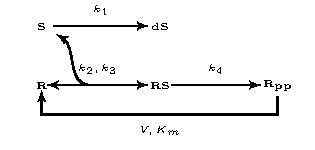
\includegraphics[clip=true,width=.42\linewidth]{experiments/diagrams/bioinformatics_model1.pdf}}
    &
    \subfigure[Modelo simplificado]{
    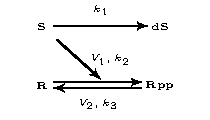
\includegraphics[clip=true,width=.42\linewidth]{experiments/diagrams/bioinformatics_model2.pdf}}
    \\
    \subfigure[Modelo incompleto] {
    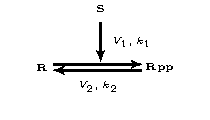
\includegraphics[clip=true,width=.42\linewidth]{experiments/diagrams/bioinformatics_model3.pdf}}
    &
    \subfigure[Modelo generalizado] {
    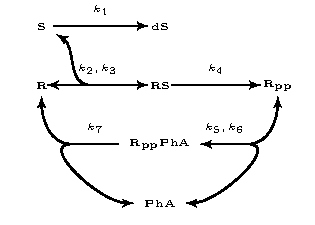
\includegraphics[clip=true,width=.42\linewidth]{experiments/diagrams/bioinformatics_model4.pdf}}
    \end{tabular}
    \caption{Os quatro modelos candidatos do primeiro experimento. A
    medida de interesse na dinâmica destes modelos é a concentração de
    R$_{pp}$.}
    \label{fig:experiment_1}
\end{figure}

No SigNetMS utilizamos 15000 iterações de burn-in e 5000 iterações para
burn-in informado e para amostragem final. Como resultado, os modelos
foram ordenados da seguinte maneira: modelo correto, modelo 
simplificado, modelo generalizado e modelo incompleto. Este resultado é
similar ao resultado original de Vyshemirsky e Girolami (2007), que tem
apenas os modelos simplificado e generalizado invertidos. Já no 
ABC-SysBio, utilizamos a sequência de limiares gerada automaticamente 
para o problema e tivemos como resultado a ordenação: modelo incompleto,
modelo simplificado, modelo generalizado e modelo correto. 

Para entender estes resultados, criamos gráficos que mostram as
simulações geradas pelos parâmetros amostrados pelo SigNetMS e
ABC-SysBio. 

Na figura~\ref{fig:exp:abc-sysbio} mostramos simulações geradas por 
amostras de parâmetros de diferentes iterações no programa ABC-SysBio, 
considerando o modelo correto. É possível ver que ao longo das iterações
os parâmetros fazem a dinâmica simulada se aproximar dos dados
experimentais. Entretanto, a dinâmica gerada pelas amostras não reproduz
a dinâmica do experimento. Isto significa que a amostra gerada pelo
programa ABC-SysBio não se aproxima da amostra da distribuição a
posteriori dos parâmetros, comprometendo a qualidade da função de
avaliação de modelos.

\begin{figure}[h]
  \centering 
  \begin{tabular}{c c}
    \subfigure[iteração 1]{
    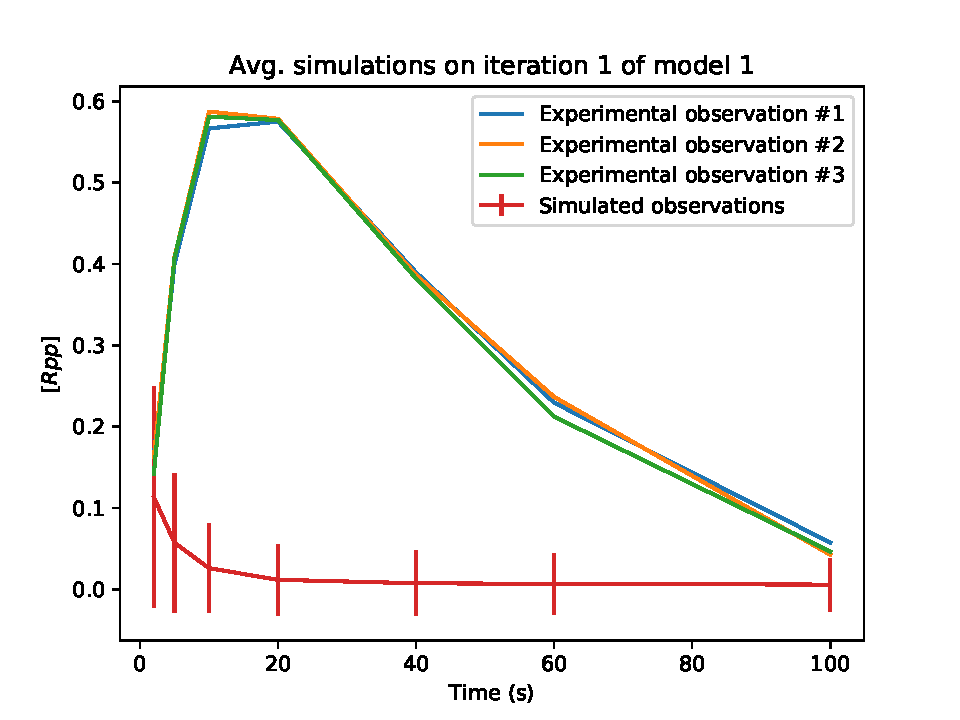
\includegraphics[clip=true,width=.45\linewidth]{experiments/results/girolami/gamma/abc/simulations_model1_1.pdf}
    \label{fig:abc_bio_avgsim1_it1}}
    &
    \subfigure[iteração 10]{
    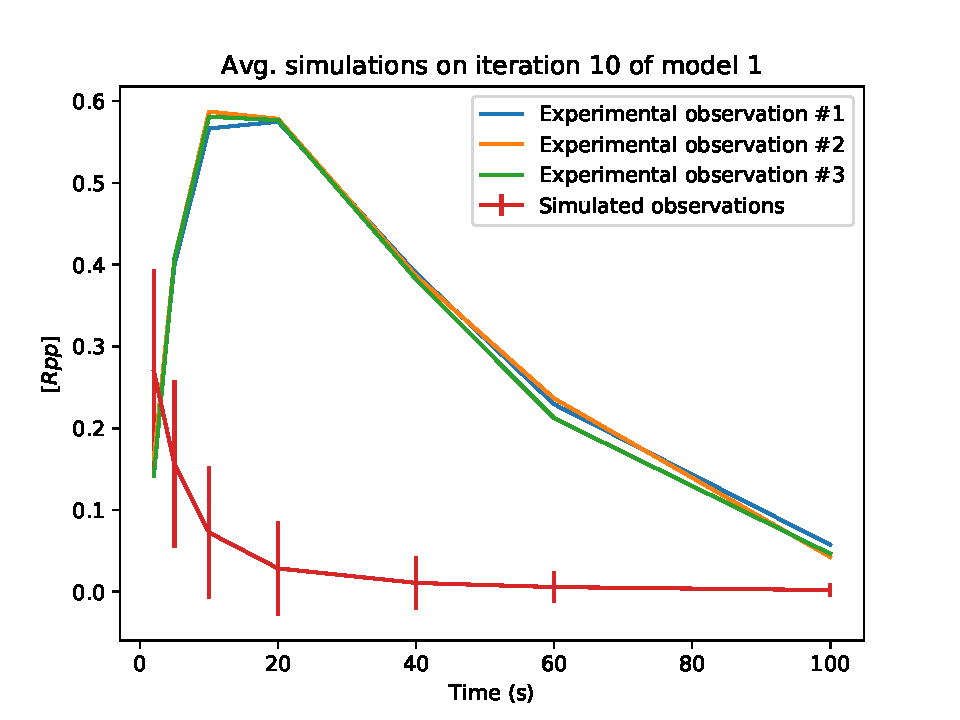
\includegraphics[clip=true,width=.45\linewidth]{experiments/results/girolami/gamma/abc/simulations_model1_10.pdf}
    \label{fig:abc_bio_avgsim1_it2}} 
    \\
      \subfigure[iteração 20]{
    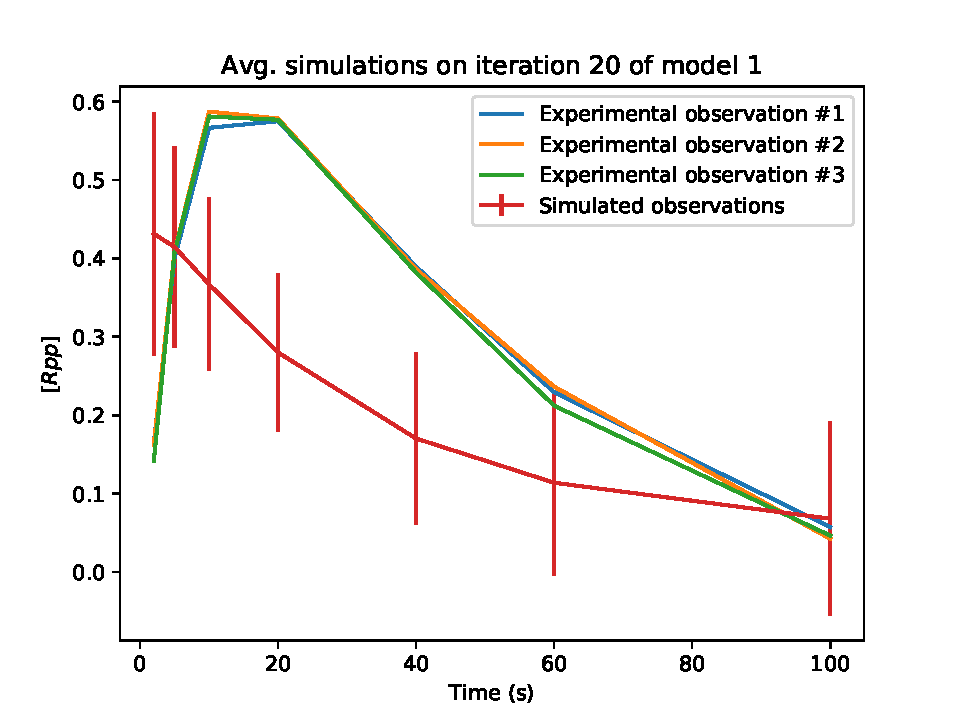
\includegraphics[clip=true,width=.45\linewidth]{experiments/results/girolami/gamma/abc/simulations_model1_20.pdf}
    \label{fig:abc_bio_avgsim1_it3}} 
    &
      \subfigure[iteração 26]{
    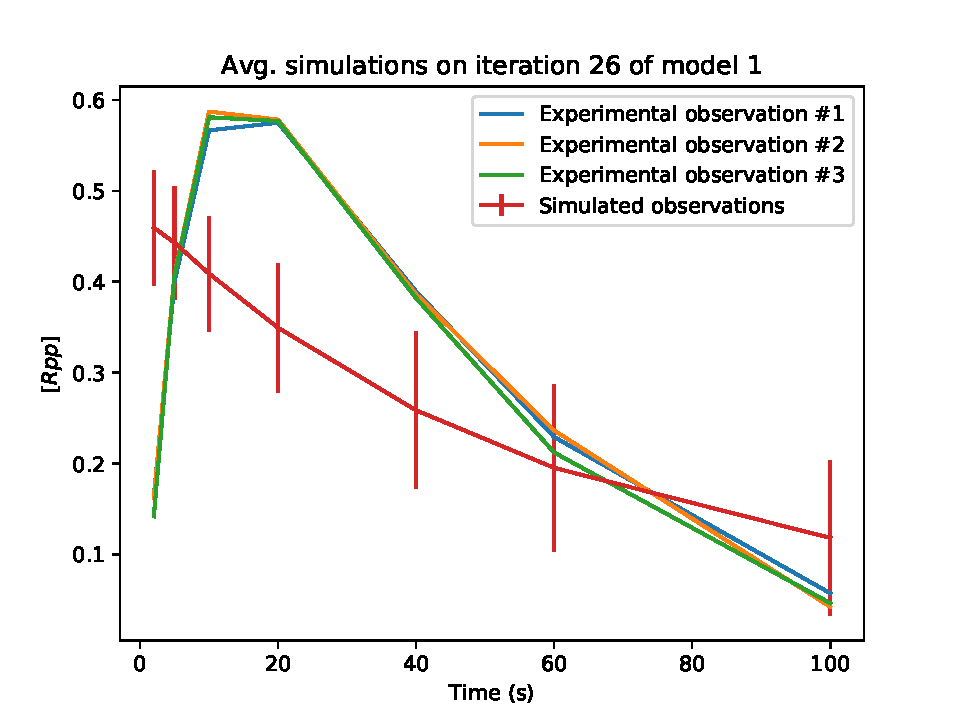
\includegraphics[clip=true,width=.45\linewidth]{experiments/results/girolami/gamma/abc/simulations_model1_26.pdf}
      \label{fig:abc_bio_avgsim1_it4}}
    \end{tabular}
    \caption{Simulação média gerada pelos parâmetros amostrados na
      iterações 1, 10, 20 e 26 pelo programa ABC-SysBio, para o modelo
      correto.}
    \label{fig:exp:abc-sysbio}
\end{figure}

Na figura~\ref{fig:exp:snm1} podemos ver simulações geradas por
parâmetros amostrados em diferentes potências de posteriori no programa
SigNetMS, considerando o modelo correto. Podemos ver que com o aumento
do valor de $\beta$, as amostras geradas se aproximam da distribuição a
posteriori, pois a curva simulada se aproxima da curva gerada no
experimento. A figura~\ref{fig:exp:snm2} mostra as simulações geradas
pelos parâmetros amostrados no SigNetMS da distribuição a posteriori, e
podemos observar que apenas o modelo incompleto, classificado como o
pior, não se aproximou da dinâmica medida no experimento. 

\begin{figure}
    \centering
    \begin{tabular}{c c}
    \subfigure[$\beta = 0$]{
    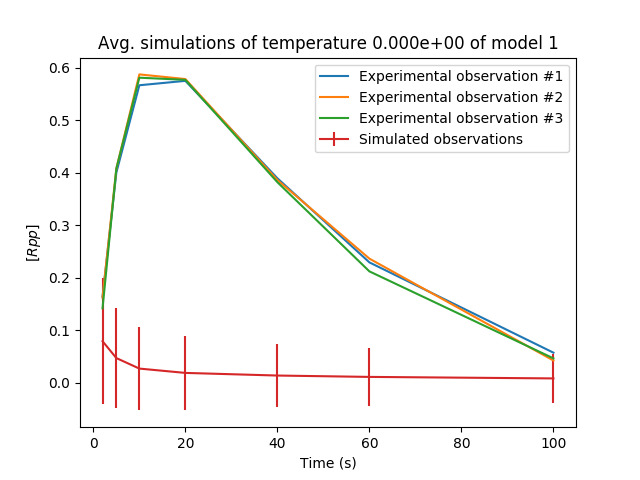
\includegraphics[clip=true,width=.45\linewidth]{experiments/results/girolami/gamma/snm/simulations_model1_0.png}
    \label{fig:abc_bio_avgsim3_it1}}
    &
    \subfigure[$\beta = 0,05$]{
    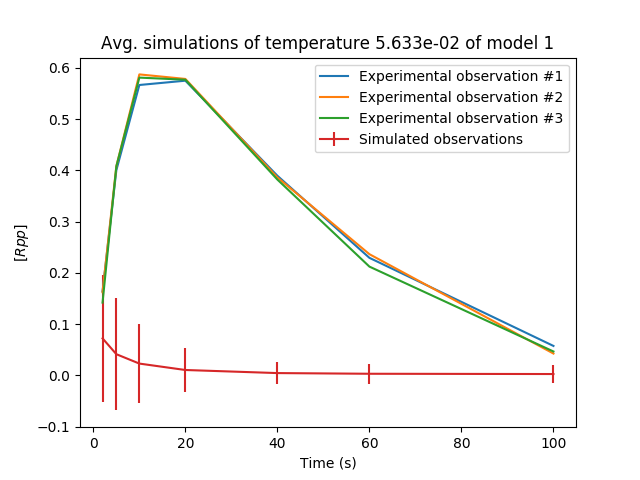
\includegraphics[clip=true,width=.45\linewidth]{experiments/results/girolami/gamma/snm/simulations_model1_19.png}
    \label{fig:abc_bio_avgsim3_it2}} 
    \\
    \subfigure[$\beta = 0,3$]{
    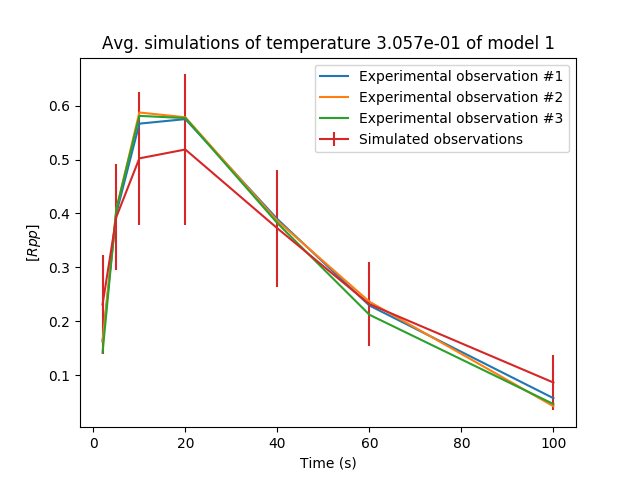
\includegraphics[clip=true,width=.45\linewidth]{experiments/results/girolami/gamma/snm/simulations_model1_29.png}
    \label{fig:abc_bio_avgsim3_it3}} 
    &
    \subfigure[$\beta = 1$]{
    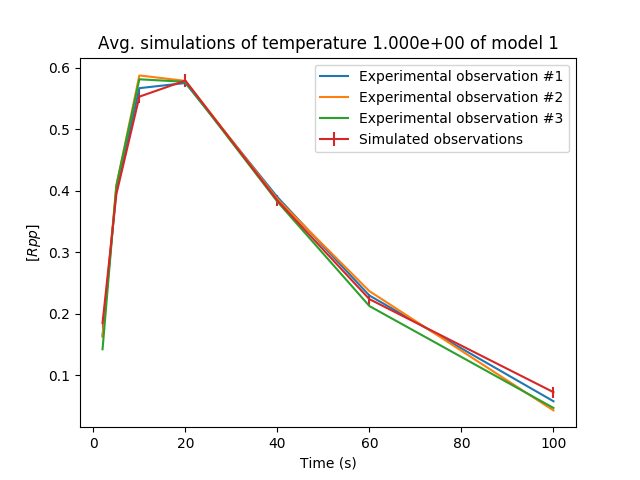
\includegraphics[clip=true,width=.45\linewidth]{experiments/results/girolami/gamma/snm/simulations_model1_39.png}
    \label{fig:abc_bio_avgsim3_it4}} 
    \end{tabular}
    \caption{Simulação média gerada pelos parâmetros amostrados no
    programa SigNetMS, para potências de posteriori com $\beta$ 
    valendo $0, 0,5, 0,3$ e $1$, para o modelo correto.}
    \label{fig:exp:snm1}
\end{figure}


\begin{figure}
    \centering
    \begin{tabular}{c c}
        \subfigure[Modelo correto]{
    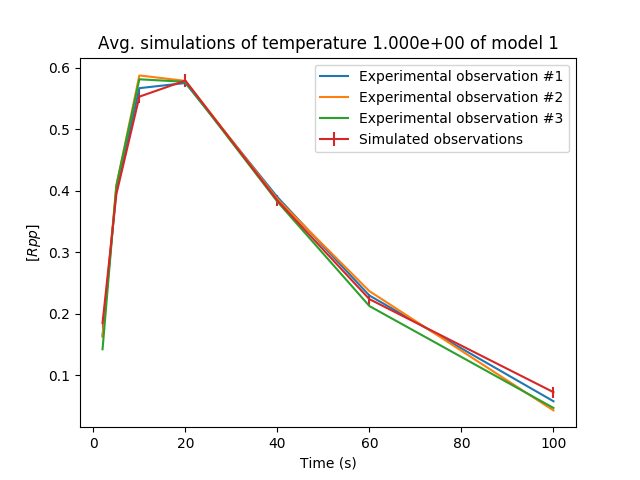
\includegraphics[clip=true,width=.46\linewidth]{experiments/results/girolami/gamma/snm/simulations_model1_39.png}}
    &
        \subfigure[Modelo simplificado]{
    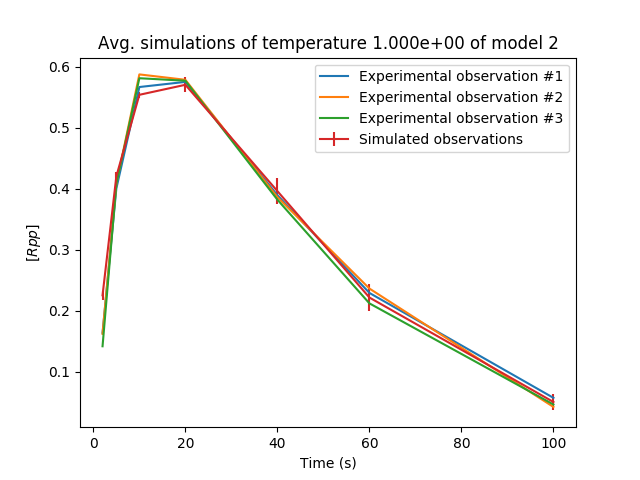
\includegraphics[clip=true,width=.46\linewidth]{experiments/results/girolami/gamma/snm/simulations_model2_39.png}} 
    \\
        \subfigure[Modelo completo]{
    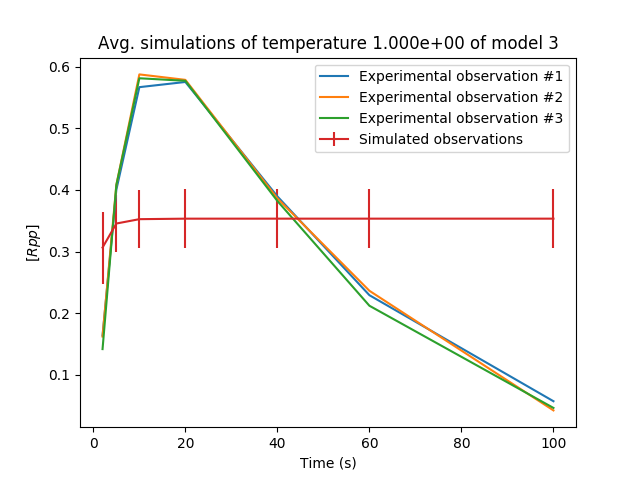
\includegraphics[clip=true,width=.46\linewidth]{experiments/results/girolami/gamma/snm/simulations_model3_39.png}} 
    &
        \subfigure[Modelo generalizado]{
    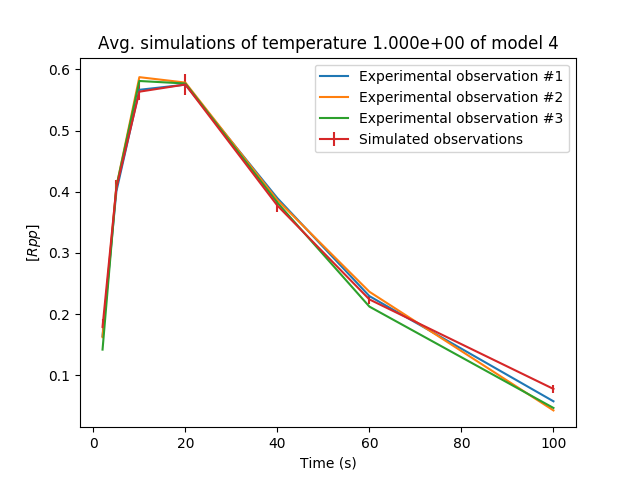
\includegraphics[clip=true,width=.46\linewidth]{experiments/results/girolami/gamma/snm/simulations_model4_39.png}} 
    \end{tabular}
    \caption{Simulação média gerada pela amostra da posteriori criada
    para os quatro modelos candidatos, no programa SigNetMS.}
    \label{fig:exp:snm2}
\end{figure}


\subsubsection{Segundo experimento}
O segundo experimento, similarmente ao primeiro, consiste em usar as
duas propostas de avaliação de modelos para criar uma ordenação de
quatro modelos em que um deles é o modelo correto, usado para geração de
dados experimentais. Os quatro modelos são apresentados da
figura~\ref{fig:experiment_2}, e são compostos, além do modelo correto,
por um modelo simplificado, por um modelo generalizado e um modelo
incorreto. 

Usando o programa ABC-SysBio obtivemos a seguinte ordenação de modelos:
modelo simplificado, modelo correto, modelo incorreto e modelo
generalizado. Por outro lado, quando utilizamos o programa SigNetMS
obtivemos a ordenação: modelo simplificado, modelo correto, modelo
generalizado e modelo incorreto.

Gerando gráficos similares ao que apresentamos no último experimento,
que mostram as simulações geradas por parâmetros amostrados, conseguimos
analisar a ordenação gerada por ambos programas. Para os modelos correto
e simplificado, ambos programas amostraram parâmetros que aproximavam a
curva simulada da curva do experimento. Para o modelo incorreto nenhum
dos dois programas amostrou parâmetros que aproximassem a dinâmica do
experimento. Por fim, para o modelo generalizado, apenas o programa
SigNetMS encontrou parâmetros que faziam a simulação aproximar os dados
do experimento.

\begin{figure}
    \centering
    \begin{tabular}{c c}
    \subfigure[Modelo correto]{
    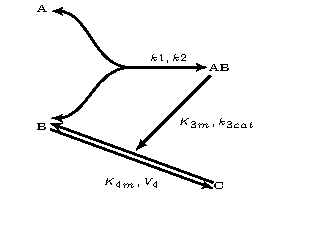
\includegraphics[clip=true,width=.4\linewidth]{experiments/diagrams/smallest_model1.pdf}}
    &
    \subfigure[Modelo simplificado]{
    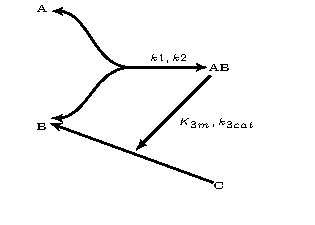
\includegraphics[clip=true,width=.4\linewidth]{experiments/diagrams/smallest_model2.pdf}} 
    \\
    \subfigure[Modelo generalizado] {
    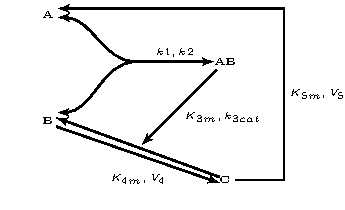
\includegraphics[clip=true,width=.4\linewidth]{experiments/diagrams/smallest_model3.pdf}}
    &
    \subfigure[Modelo incorreto] {
    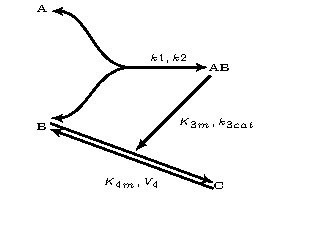
\includegraphics[clip=true,width=.4\linewidth]{experiments/diagrams/smallest_model4.pdf}} 
    \end{tabular}
    \caption{Os quatro modelos candidatos no segundo experimento. A
    medida de interesse nestas vias é a concentração de C.}
    \label{fig:experiment_2}
\end{figure}

\subsubsection{Escolha de método de avaliação de modelos}
Com os resultados obtidos nos dois experimentos anteriores, concluímos
que a ferramenta SigNetMS é mais adequada para nossas aplicações do que
a ferramenta ABC-SysBio. É importante também ressaltar que a ferramenta
ABC-SysBio pode ser mais adequada em aplicações em que uma função de
verossimilhança não pode ser escrita, e também em situações em que é
difícil determinar uma distribuição a priori para constantes de
velocidade. 

\subsection{Paralelização do SigNetMS}
Apesar de se mostrar mais adequada para nossas aplicações, a ferramenta
SigNetMS possuia como grande desvantagem o seu tempo de execução. Por
conta disto, analisamos a ferramenta com objetivo de identificar porções 
de código que poderiam ser executadas em paralelo. Identificamos então
que o procedimento de geração de amostras de potências de posteriori era 
responsável por grande parte do tempo de execução.

O procedimento de geração de amostras foi implementado com o algoritmo
de Metropolis-Hastings, que é de difícil paralelização, pois um passo
depende do passo anterior. Entretanto, as amostras de diferentes
potências de posteriori são geradas de maneira independente nas etapas
de burn-in e burn-in informado. Logo, paralelizamos estas duas etapas da
amostragem. Para implementar a paralelização utilizamos a biblioteca
\toolname{pathos}\footnote{https://github.com/uqfoundation/pathos},
e a função \toolname{map}, que nos permitiu fazer com que cada potência
de posteriori fosse amostrada, nas etapas de burn-in e burn-in
informado, em uma thread diferente.

A última etapa do processo de amostragem não foi paralelizada, pois nela
é realizado o processo de Monte Carlo Markov Chain
Populacional~\cite{Friel2008}, que mistura amostras de diferentes
potências de posteriori, dificultando a paralelização.

\subsection{Implementação eficiente de integração de sistemas de
equações diferenciais}
Mesmo com a paralelização do processo de amostragem, o tempo de execução
do programa SigNetMS ainda era muito grande, mesmo para exemplos
pequenos. Decidimos então investigar o processo de integração de sistema
de equações diferenciais.

Até este momento, estávamos usando uma representação literal do sistema
de equações diferenciais. Portanto, para fazer sua integração, usávamos
uma função que interpretava as derivadas em formato texto e calculava 
seus respectivos valores. Propomos então, utilizar uma notação simbólica 
do sistema de equações diferenciais, utilizando a biblioteca 
\toolname{SymPy}. 

Ao utilizar a notação simbólica no SymPy, fomos capazes de usar funções
da própria biblioteca que permitem transformar o sistema de equações
diferenciais em uma função escrita em C, que é automaticamente compilada
e transformada em uma função em Python. Além disso, a notação simbólica
também nos permite facilmente calcular a matriz Jacobiana do sistema de
equações diferenciais, o que melhora o desempenho do integrador
numérico. A tabela~\ref{tab:integrador} mostra o tempo de execução do
integrador numérico quando usamos as duas diferentes abordagens de
representação do sistema, e é possível ver que com a notação simbólica,
o tempo de execução diminuiu consideravelmente.

\begin{table}[]
\centering
\begin{tabular}{ccc}
\hline
\multicolumn{1}{l}{}  & \multicolumn{2}{c}{Tempo de execução em segundos} \\ 
\hline

\multicolumn{1}{l}{\# de integrações do sistema}
    & Representação literal  & Representação simbólica  \\
\hline
100 & 31,1  & 5,4  \\
200 & 63,3  & 10,5 \\
400 & 125,6 & 20,3 \\ 
\hline
\end{tabular}
\caption{Tempo de execução do integrador numérico usando as duas
    abordagens de representação do sistema de equações diferenciais.
    Para gerar esta tabela, o modelo correto da
    figura~\ref{fig:experiment_1} foi integrado numericamente repetidas 
    vezes.}
\label{tab:integrador}
\end{table}

\subsection{Testes da metodologia em uma cadeia do espaço de busca} 
Com a melhora de desempenho do pacote SigNetMS, seguimos o trabalho com
um experimento maior de seleção de via de sinalização celular. Este
experimento consistiu em adicionar, uma a uma e de maneira aleatória, 
reações candidatas a um modelo inicial e analisar o comportamento da 
função de custo sobre sequência de modelos criada. Do ponto de vista de
seleção de características (em que reações candidatas são
características), este experimento é equivalente a um passeio aleatório
no espaço de busca (todos os subconjuntos de características) que sempre
adiciona características, começando no conjunto vazio, correspondente ao
modelo base, e terminando no conjunto completo, correspondente ao modelo
base mais todas as reações candidatas.

Os dados experimentais para avaliação dos modelos foram gerados por um
modelo intermediário, entre o modelo base e o modelo com conjunto
completo de reações. A figura~\ref{fig:random_walk} mostra o resultado 
deste experimento, e nela podemos ver que a função de custo de fato 
penaliza modelos mais complexos, e que a função de custo não é 
monotônica em uma cadeia do espaço de busca e também não tem um formato
de U, o que vai influenciar na nossa escolha por um algoritmo de busca.

\begin{figure}
    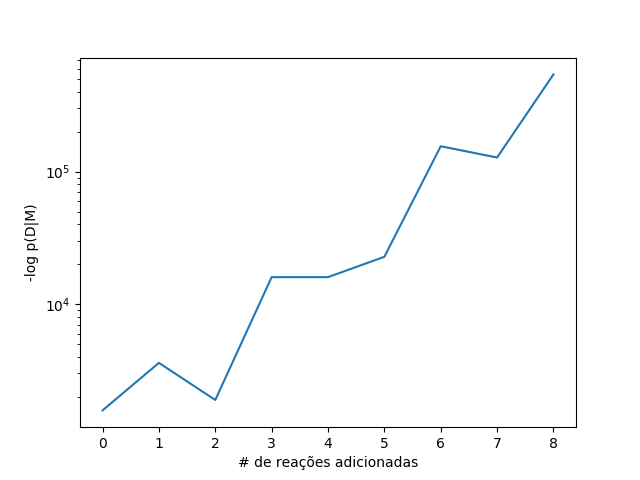
\includegraphics[clip=true]{experiments/surface_curve.png}
    \caption{Curva com comportamento da função de custo ao adicionar
    iterativamente reações a um modelo base. Para facilitar a
    visualização, mostramos no gráfico a verossimilhança marginal vezes 
    a constante $-1$, ou seja, quanto menor o valor na curva, melhor a
    qualidade do modelo. 
    }
    \label{fig:random_walk}
\end{figure}

\section{Atividades futuras}
Nos mês de fevereiro, projetamos finalizar experimentos de percorrimento
do espaço de busca. Em seguida, nos meses de março, abril e maio
projetamos construir um pequeno banco de dados de reações químicas,
e aplicar a metodologia proposta em linhagens de células Y1 e HEK293.

\section{Outras atividades acadêmicas}
No mês de janeiro de 2019, entre os dias 7 e 11, o beneficiário 
participou da XIV Escuela de Verano en Matemáticas Discretas, em 
Valparaíso, Chile. Nesta escola três cursos foram oferecidos, envolvendo
otimização combinatória, análise de algoritmos parametrizados e
problemas computacionais no estudo do cérebro.

Além disso, o beneficiário teve um resumo aceito para participação na
conferência Rocky 2019. O beneficiário participou da conferência entre
os dias 5 e 7 de dezembro, na cidade Snowmass Village, Colorado, Estados
Unidos. Esta conferência possuiu uma seção de posters na qual o
beneficiário apresentou o trabalho desenvolvido neste projeto.

\addcontentsline{toc}{section}{Referências}
\bibliographystyle{unsrt} 
\bibliography{bib-relatorio}
\end{document}
